\documentclass[10pt,twocolumn,letterpaper]{article}

\usepackage{cvpr}
\usepackage{times}
\usepackage{epsfig}
\usepackage{graphicx}
\usepackage{amsmath}
\usepackage{amssymb}
\usepackage{graphicx}
\usepackage[utf8]{inputenc}
\usepackage[T1]{fontenc}
\usepackage{lmodern} % load a font with all the characters
\usepackage[justification=centering]{caption}
\usepackage{float}
\usepackage{enumitem}
\usepackage{caption}
\usepackage{lipsum}
\usepackage{titlesec}
\captionsetup[figure]{name=Figura}
\captionsetup[table]{name=Tabla}
% Include other packages here, before hyperref.

% If you comment hyperref and then uncomment it, you should delete
% egpaper.aux before re-running latex.  (Or just hit 'q' on the first latex
% run, let it finish, and you should be clear).
%\usepackage[breaklinks=true,bookmarks=false]{hyperref}

\cvprfinalcopy % *** Uncomment this line for the final submission

\def\cvprPaperID{****} % *** Enter the CVPR Paper ID here
\def\httilde{\mbox{\tt\raisebox{-.5ex}{\symbol{126}}}}

% Pages are numbered in submission mode, and unnumbered in camera-ready
%\ifcvprfinal\pagestyle{empty}\fi
\setcounter{page}{1}
\begin{document}

%%%%%%%%% TITLE
\title{Clasificación de Pirámides de Histogramas de Palabras (PHOW)}

\author{Juliana de la Vega Fernández\\
código 201312387\\
Departamento de Ingeniería Biomédica\\
Universidad de los Andes\\
{\tt\small j.de10@uniandes.edu.co}}

\maketitle
%\thispagestyle{empty}

%%%%%%%%% ABSTRACT
\begin{abstract}
   En este artículos se presentan los resultados obtenidos a partir de la implementación de la base de datos tiny de imagenet en el código de Caltech para realizar PHOW (Pyramid Histogram of Words). Aunque el código fue elaborado para la base de datos caltech101, se experimenta con una base de datos de mayor complejidad buscando analizar el funcionamiento de la representación realizada mediante PHOW. Posteriormente se realiza una clasificación mediante un support vector machine. Particularmente se observa cómo afecta en el resultado final las variaciones en el número de categorías entrenadas, la cantidad de imágenes empleadas en el entrenamiento, y las particiones espaciales.
\end{abstract}

%%%%%%%%% BODY TEXT
\section{\textbf{I. Introducción}}

PHOW o \textit{Bag of Words} es uno se los algoritmos mas sencillos para el reconocimiento de categorías. Este algoritmo calcula la distribución, representada por el histograma, de palabras visuales encontradas en la imagen de prueba comparándola con la distribución de las palabras en la base de entrenamiento [1]. Usualmente se emplea SIFT, o \textit{Scale Invariant Feature Transform} como descriptor de las imágenes. Como tal, los descriptores de SIFT se forman al calcular el gradiente en cada pixel en una ventana de 16 x 16 píxeles alrededor del pixel central, empleando el nivel adecuado de la pirámide gaussiana en el cual el pixel central fue detectado. El gradiente de las magnitudes pierde peso de acuerdo a una función gaussiana de decaída [1]. En la totalidad de una imagen se pueden formar un vector descriptor SIFT con 128 valores. 

\subsection{\textit{A. Base de Datos: Caltech101}}

Inicialmente, PHOW fue empleada sobre la base de datos de caltech101 del California Technical Institute, sin embargo luego resultó evidente que la base de datos del caltech101 resultaba poco realista en cuanto a que empleaba 101 categorias, cada una con 50 imágenes, y con tamaños de 300x200 píxeles [2]. Usualmente estas imágenes presentan un único objeto centrado, sin ruido, en un fondo fácilmente distinguible. Adicionalmente, las imágenes se encuentran es posiciones estereotípicas [2]. Tres ejemplos de categorías de la base de datos se pueden observar en la figura 1.
\begin{figure}
\begin{center}
   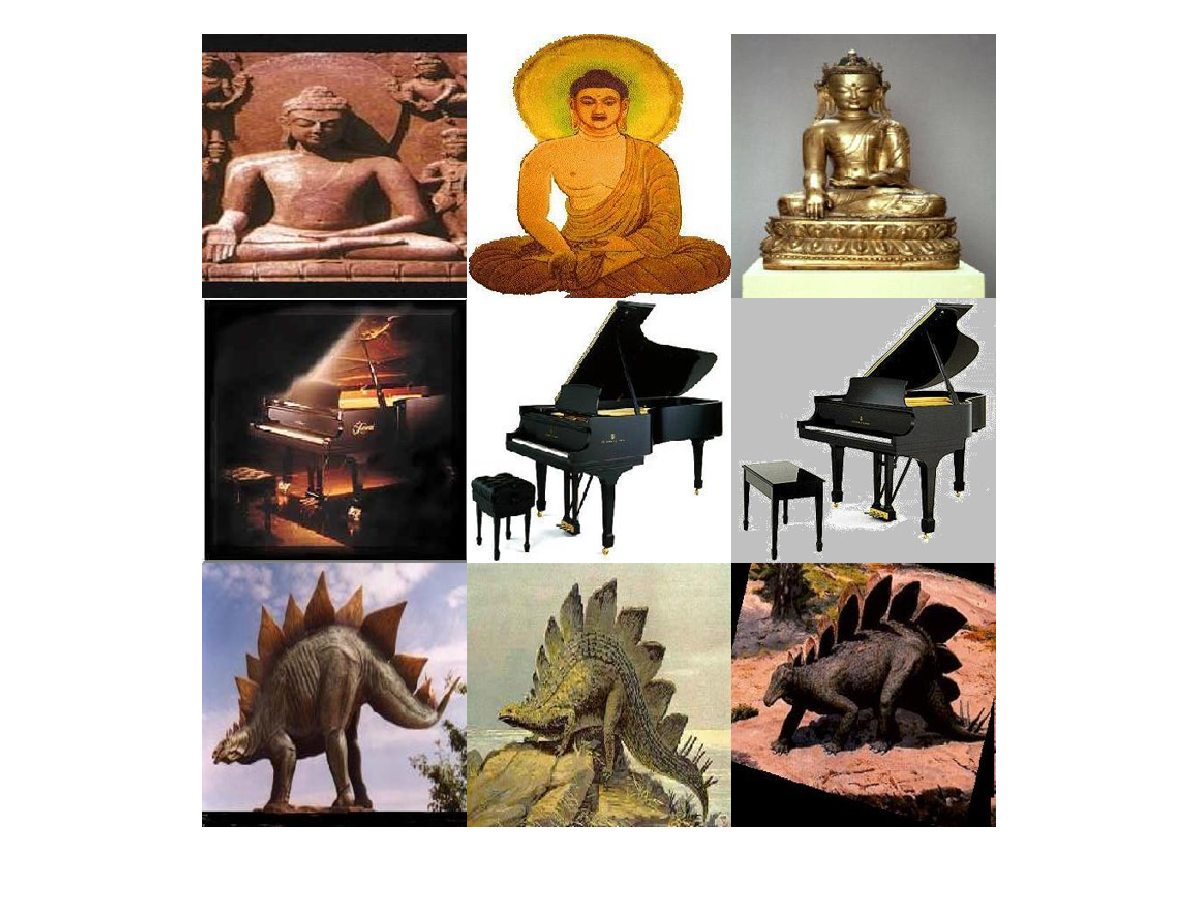
\includegraphics[scale = 0.4]{fig1PHOW}
\end{center}
   \caption{Ejemplos de las categorias Buddha, grandpiano y stegosaurus de la base de datos Caltech-101.}
\end{figure}

\subsection{\textit{B. Base de Datos: Imagenet Tiny}}

Luego de reconocer los problemas básicos de la base de datos Caltech101, se desarrollaron nuevas bases de datos con imágenes reales, con objetos en todas las posiciones, varios objetos en una imagen, y ruido de en el fondo. Una de estas bases de datos corresponde a la base Imagenet. Particularmente, el subgrupo Tiny cuenta con 200 categorías, cada una con 100 imágenes de 256x256 píxeles, en escala RGB y formato JPEG. En la figura 2 se puede observar un ejemplo de 3 imágenes de 3 categorías. Como se observa, los objetos están en diferentes posiciones  y son bastante variados dentro de la misma categoría. En el ejemplo se observan tres ejemplos de las categorías: carros de golf, bananos y comadrejas

\begin{figure}
\begin{center}
   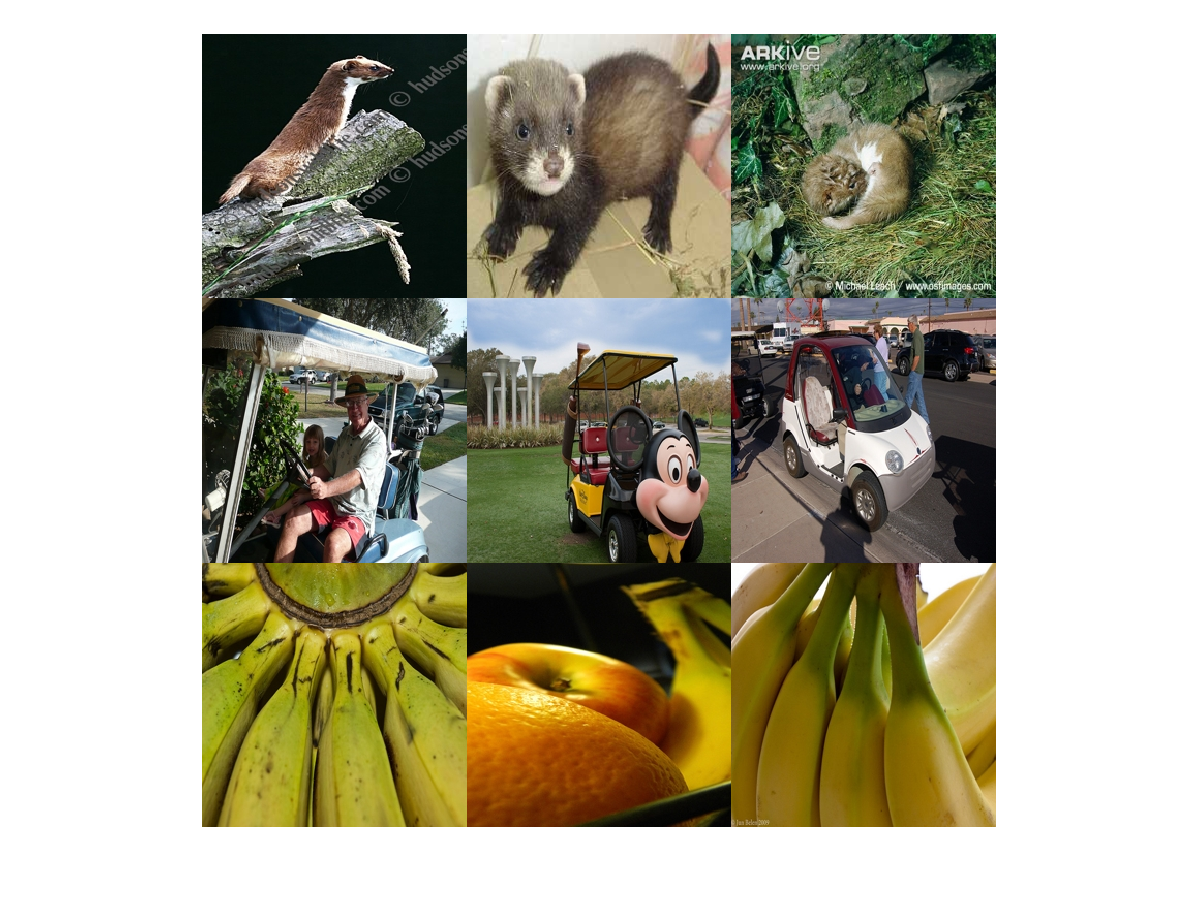
\includegraphics[scale = 0.4]{fig2PHOW}
\end{center}
   \caption{Ejemplos de las categorias weasel, golfcart y banana de la base de datos Imagenet Tiny.}
\end{figure}

\section{\textbf{II. Metodología}}

Para el desarrollo del laboratorio se emplea la biblioteca VLFeat para Matlab [3]. Esta biblioteca contiene algoritmos útiles para las tareas de visión por computador. Como tal se empleará el código para SIFT. También se emplea como base el código de Andrea Vedaldi \textit{phow\_caltech101.m} donde se implementa PHOW mediante SIFT, y se realiza clasificación empleando un support vector machine para la base de datos caltech. 

\subsection{\textit{A. Adaptación del código a la base de datos Imagenet tiny}}

Se realizaron pequeñas modificaciones al código original para que este funcionara en la base de datos imagenet tiny. Inicialmente, se cambian los directorios \textit{conf.calDir}, donde se encuentran las imágenes de entrenamiento, y \textit{conf.dataDir}, donde se almacenarán los datos del modelo desarrollado. La variable \textit{conf.autoDownloadData} se cambia a false para que no se descarguen las imágenes de caltech, debido a que estas no se van a emplear. 

En la sección del código destinada a descargar los datos de Caltech-101 se modifican unos ciclos condicionales \textit{if} para que verificaran la existencia de la carpeta \textit{agaric} que corresponde a una categoría de las imágenes de la base de datos imagenet tiny. También se comenta la parte del código que realiza la descarga y descompresión de las imágenes de Caltech-101.

En la sección del código denominada \textit{Setup data} se cambia un aspecto de la variable \textit{ims} dentro de un ciclo \textit{for}, para que esta variable encuentre los archivos cuyo formato es \textit{JPEG} en lugar de \textit{JPG}. Por último, se agregan variables de medición de tiempos a lo largo del código para realizar análisis con relación a la duración del entrenamiento, la clasificación y la prueba del mismo al cambiar ciertas variables. 

\subsection{ \textit{B. Funcionamiento del código}}
A continuación se describe brevemente el funcionamiento del código. 

\subsubsection*{Descriptores}
Inicialmente se obtienen los descriptores de tipo SIFT de las imágenes de entrenamiento. Con estos descriptores se entrena el diccionario, y mediante \textit{k-means} se organiza el diccionario en 600 palabras o clústeres.

\subsubsection*{Representación}
Una vez se tenga el diccionario de palabras, se representan las imágenes de entrenamiento empleando el método PHOW, asociando palabras del diccionario a cada una de las imágenes de la base de datos de entrenamiento. Cada imagen estará representada por un vector de tamaño 600 que contiene la descripción de las palabras visuales encontradas en la imagen.

\subsubsection*{Clasificación}
Para la clasificación se emplea un support vector machine, con el cual se obtiene un modelo para clasificar las imágenes en la base de datos de prueba. 
\subsubsection*{Evaluación}
Por último, se introducen los descriptores SIFT de las imágenes de la base de datos de prueba en el modelo entrenado para predecir la categoría a la cual pertenecen.

\subsection{ \textit{C. Variación de parámetros}}
El código descrito anteriormente fue modificado en las variables \textit{conf.numTrain}, \textit{conf.numClasses}, y \textit{conf.numSpatialX} con el objetivo de examinar los cambios en la precisión al variar una de las anterior de manera independientemente. La variable \textit{conf.numTrain} se examinó con valores de 15, 30 y 50 imágenes de entrenamiento; la variable \textit{conf.numClasses} se examinó en valores de 25, 50, 100 y 200 categorías; y la variable {conf.numSpatialX} se examinó con valores de [1,2], [2,4] y [8,16].


\section{\textbf{ III. Resultados}}
A continuación se presentan los resultados obtenidos con los modelos entrenados empleando PHOW en la base de datos Imagenet Tiny. Para obtenerlos se realizaron 9 diferentes modelos de entrenamiento. 
\begin{itemize}
  \item Modelo con 25 categorías, 50 imágenes de entrenamiento y variable espacial [1,2]. (figura 3)
  \item Modelo con 25 categorías, 50 imágenes de entrenamiento y variable espacial [2,4]. (figura 4)
  \item Modelo con 25 categorías, 50 imágenes de entrenamiento y variable espacial [8,16]. (figura 5)
  \item Modelo con 50 categorías, 50 imágenes de entrenamiento y variable espacial [2,4]. (figura 6)
  \item Modelo con 100 categorías, 50 imágenes de entrenamiento y variable espacial [2,4]. (figura 7)
  \item Modelo con 200 categorías, 50 imágenes de entrenamiento y variable espacial [2,4]. (figura 8)
  \item Modelo con 200 categorías, 15 imágenes de entrenamiento y variable espacial [2,4]. (figura 9)
  \item Modelo con 200 categorías, 30 imágenes de entrenamiento y variable espacial [2,4]. (figura 10)
  \item Modelo con 200 categorías, 100 imágenes de entrenamiento y variable espacial [2,4].
\end{itemize}

Cada modelo cuenta con su propia matriz de confusiones exhibiendo sus resultados, a excepción del modelo con 200 categorías, 100 imágenes de entrenamiento y variable espacial [2,4] debido a que ese representa el modelo del punto bono. 

\begin{figure}
\begin{center}
   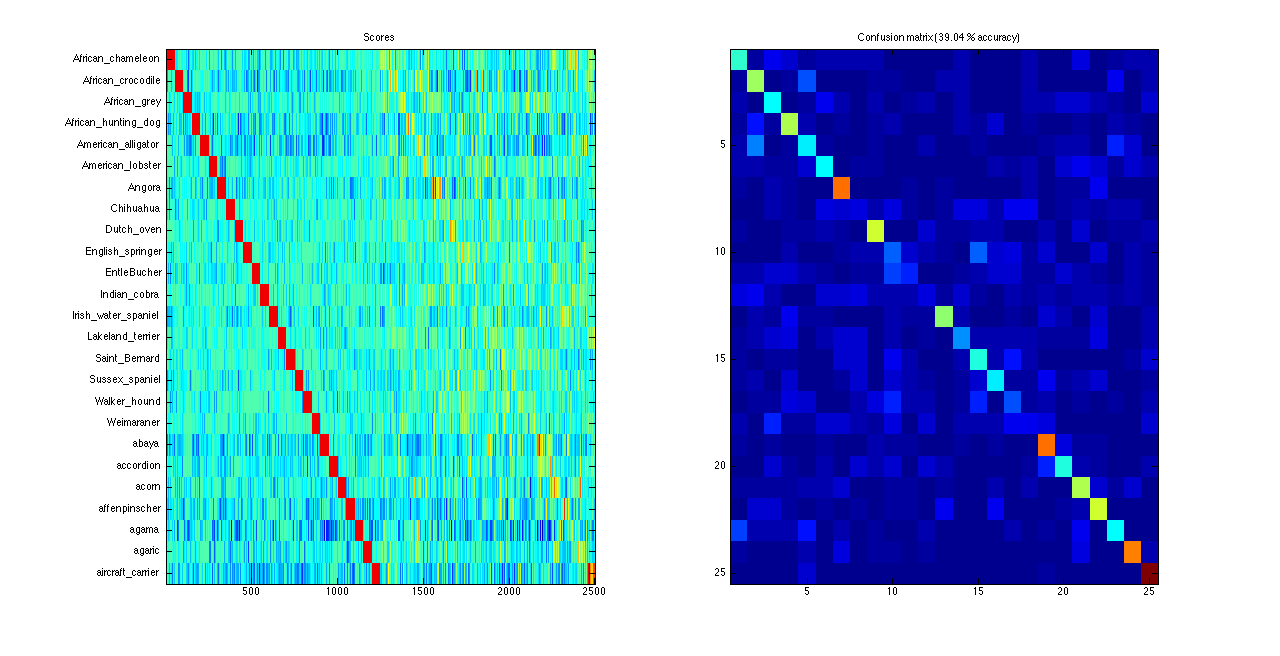
\includegraphics[scale = 0.2]{255012ConfusionMatrix}
\end{center}
   \caption{Matriz de confusiones para el modelo con 25 categorías, 50 imágenes de entrenamiento y variable espacial [1,2].}
\end{figure}

\begin{figure}
\begin{center}
   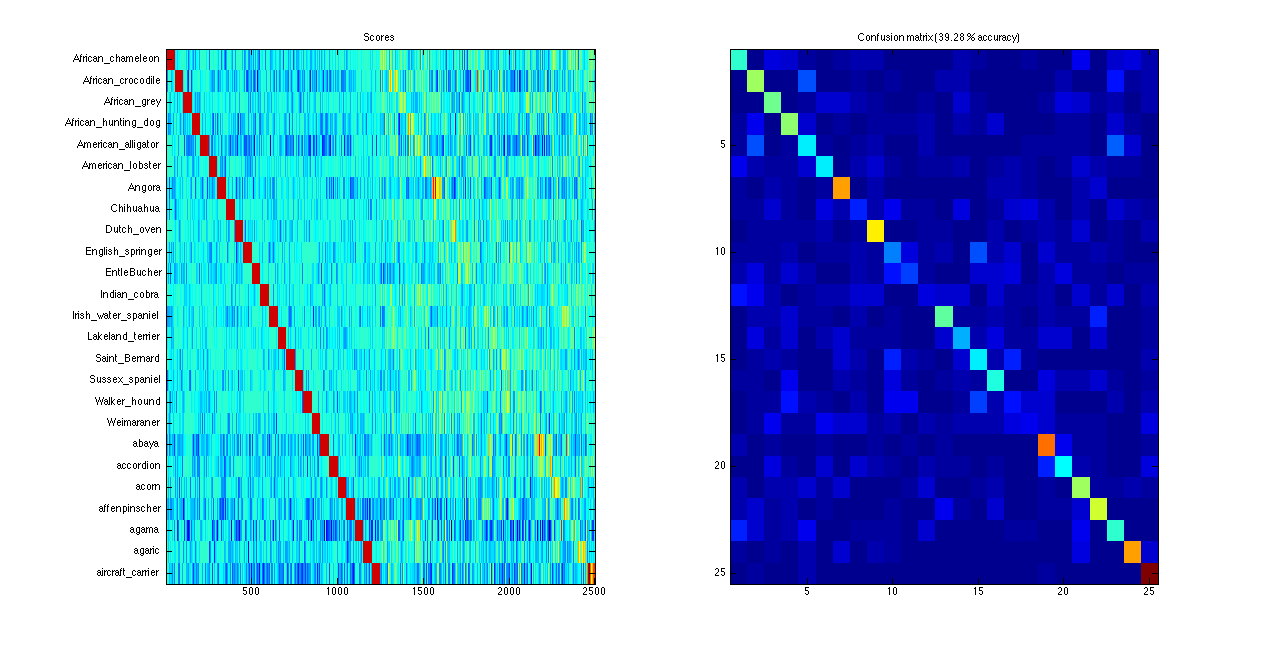
\includegraphics[scale = 0.2]{255024ConfusionMatrix} 
\end{center}
   \caption{Matriz de confusiones para el modelo con 25 categorías, 50 imágenes de entrenamiento y variable espacial [2,4].}
\end{figure}

\begin{figure}
\begin{center}
   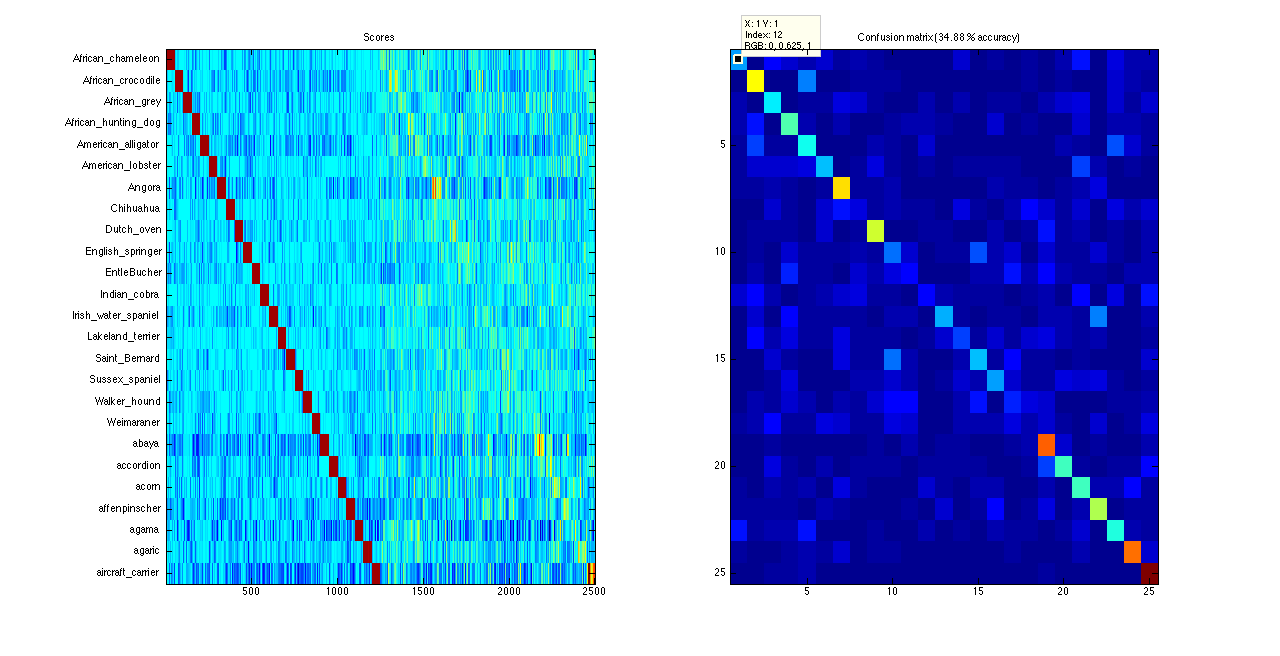
\includegraphics[scale = 0.2]{2550816ConfusionMatrix}
\end{center}
   \caption{Matriz de confusiones para el modelo con 25 categorías, 50 imágenes de entrenamiento y variable espacial [8,16].}
\end{figure}

\begin{figure}
\begin{center}
   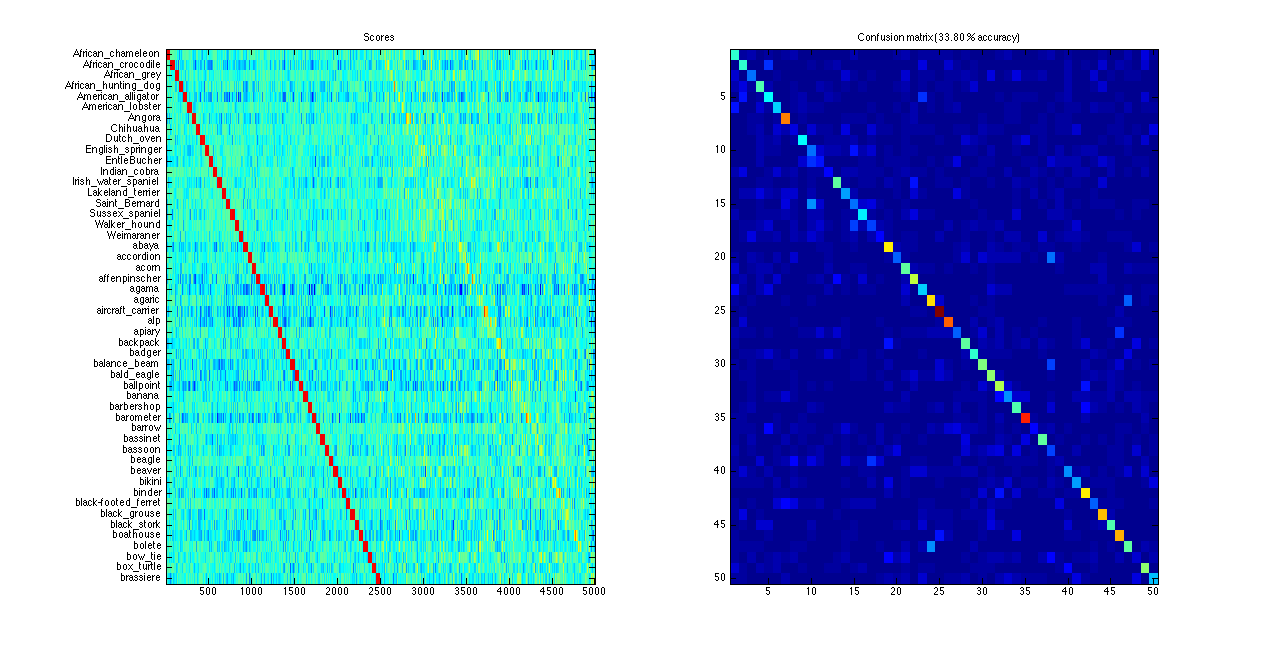
\includegraphics[scale = 0.2]{505024ConfusionMatrix}
\end{center}
   \caption{Matriz de confusiones para el modelo con 50 categorías, 50 imágenes de entrenamiento y variable espacial [2,4].}
\end{figure}

\begin{figure}
\begin{center}
   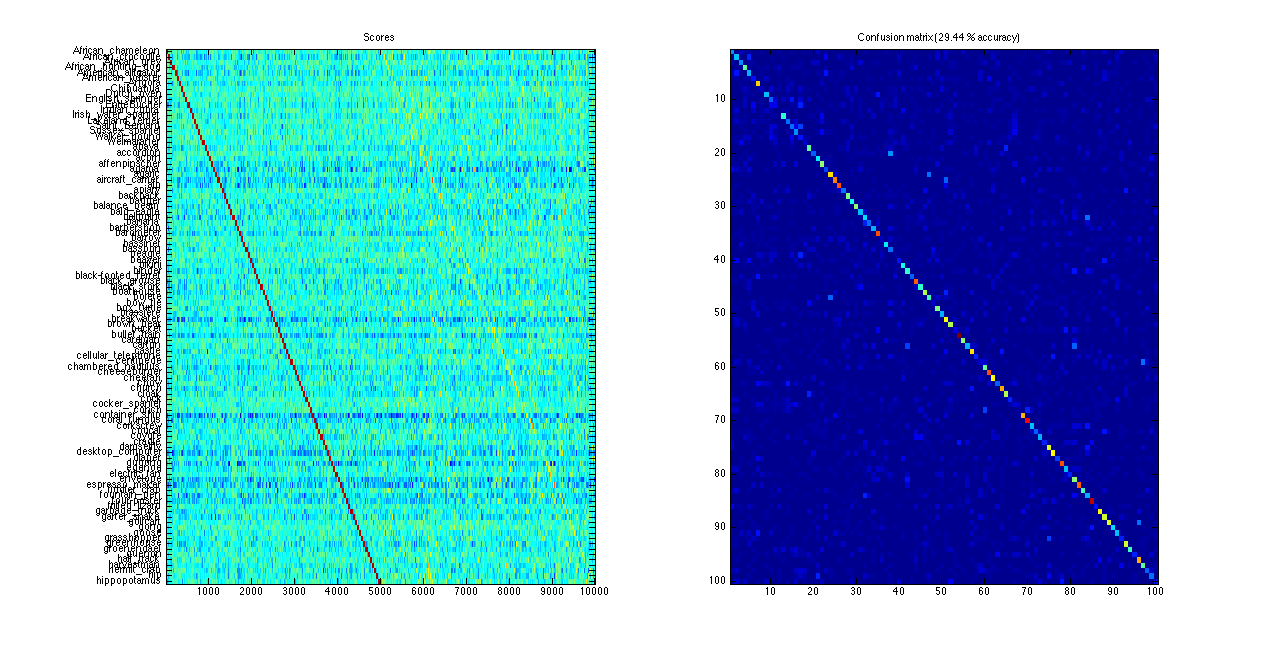
\includegraphics[scale = 0.2]{1005024ConfusionMatrix}
\end{center}
   \caption{Matriz de confusiones para el modelo con 100 categorías, 50 imágenes de entrenamiento y variable espacial [2,4].}
\end{figure}

\begin{figure}
\begin{center}
   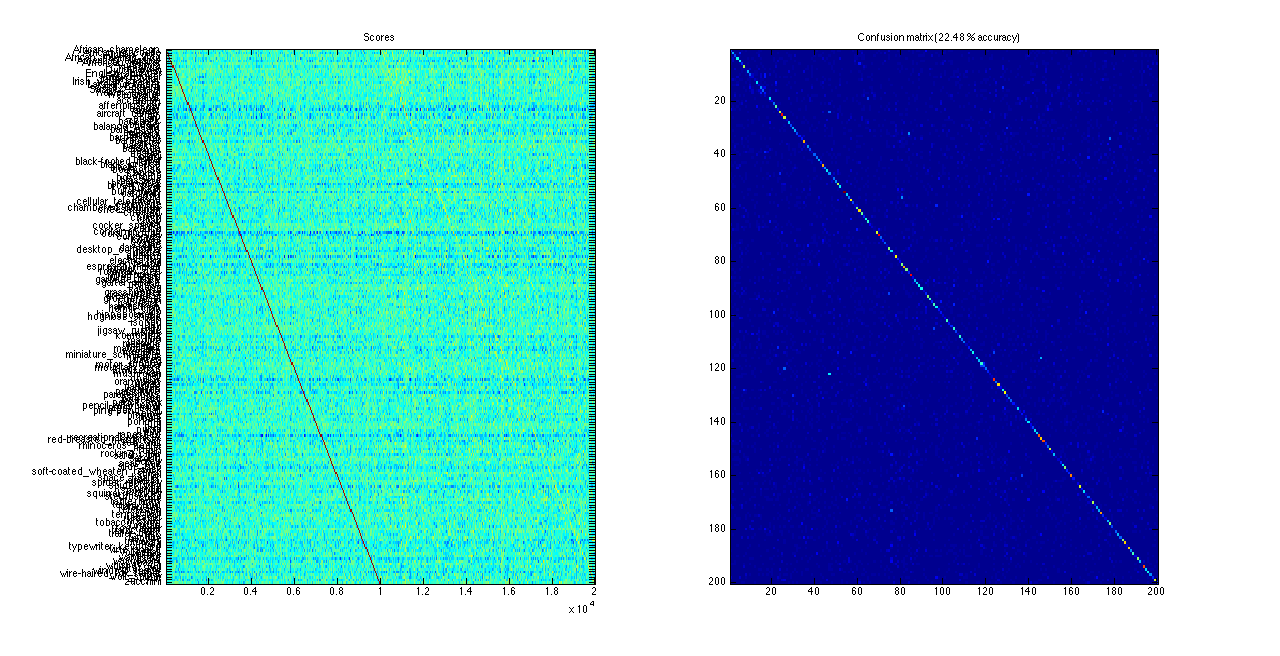
\includegraphics[scale = 0.2]{2005024ConfusionMatrix}
\end{center}
   \caption{Matriz de confusiones para el modelo con 200 categorías, 50 imágenes de entrenamiento y variable espacial [2,4].}
\end{figure}

\begin{figure}
\begin{center}
   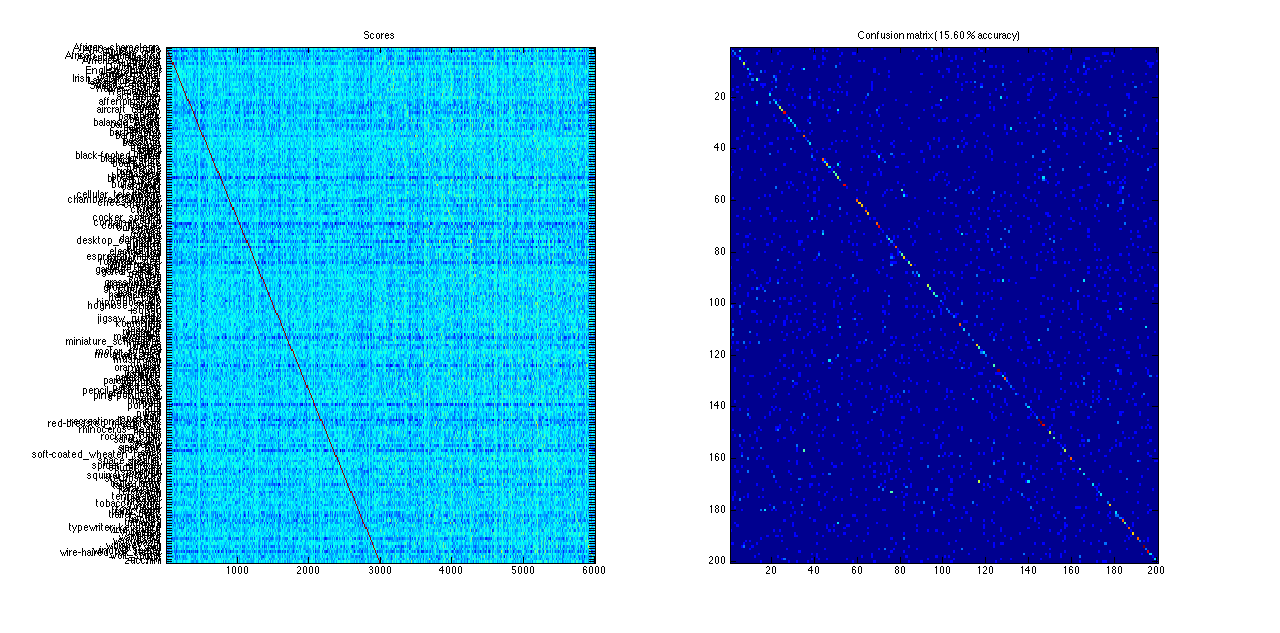
\includegraphics[scale = 0.2]{2001524ConfusionMatrix}
\end{center}
   \caption{Matriz de confusiones para el modelo con 200 categorías, 15 imágenes de entrenamiento y variable espacial [2,4].}
\end{figure}

\begin{figure}
\begin{center}
   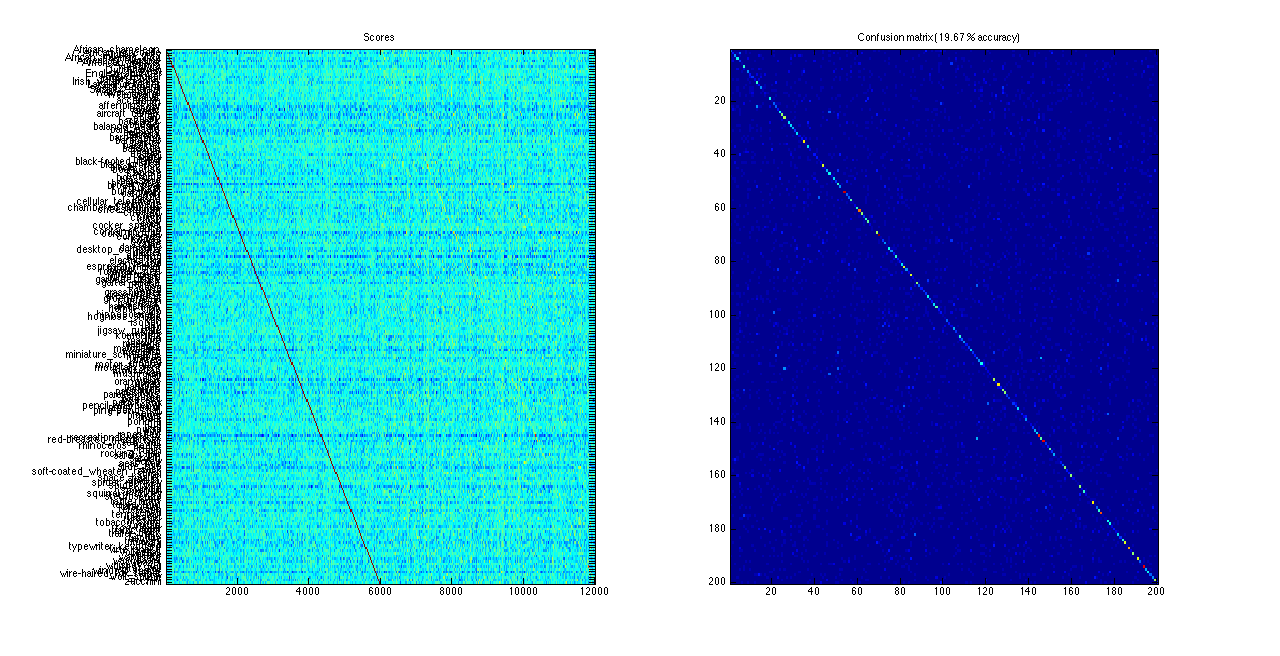
\includegraphics[scale = 0.2]{2003024CorrelationMatrix}
\end{center}
   \caption{Matriz de confusiones para el modelo con 200 categorías, 30 imágenes de entrenamiento y variable espacial [2,4].}
\end{figure}

\subsection{ \textit{A. Spatial X}}

Para evaluar la variable \textit{conf.numSpatialX} se utilizan los modelos con 25 categorías, 50 imágenes de entrenamiento y con configuraciones espaciales de [1,2], [2,4] y [8,16] debido a que en estos modelos solo cambia la variable que se está evaluando. En la figura 11 se puede apreciar cómo varía precisión del modelo de acuerdo con los cambios de la variable espacial.

\begin{figure}
\begin{center}
   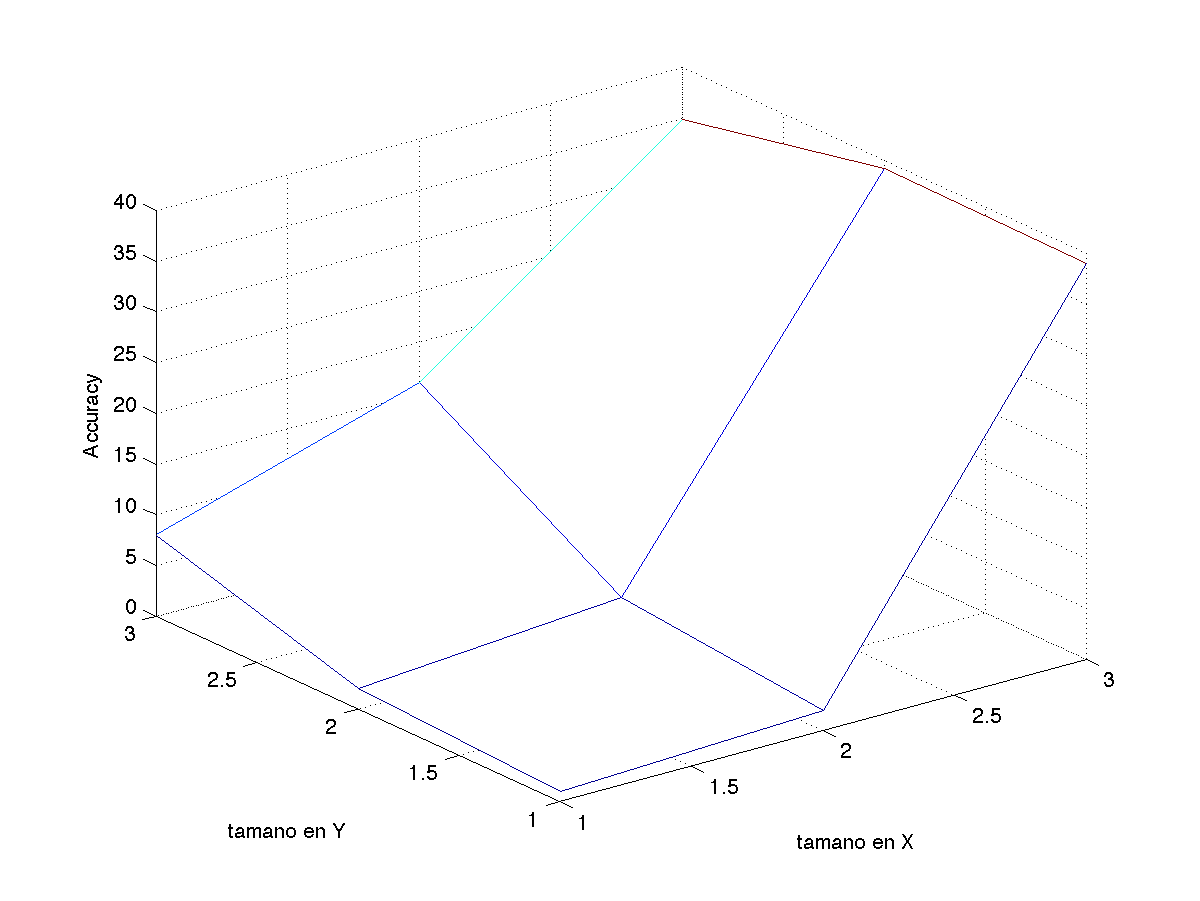
\includegraphics[scale = 0.4]{fig5spatialPHOW}
\end{center}
   \caption{Gráfica de precisión contra las configuraciones espaciales en X.}
\end{figure}

La precisión para el caso en el que se utiliza la configuración espacial [1,2] es de 39.04\%, para el caso con configuración [2,4] corresponde a 39.28\%, y para el caso de [8,16] corresponde a 34.88\%. Adicionalmente, se presentan los tiempos de procesamiento comparativos en la tabla 1, presentando las diferencias en cuanto a segundos al emplear los diferentes modelos para evaluar cómo influye la variable de la configuración espacial.

%-----------------Tabla Spatial X
\begin{table*}
\caption{Tiempos comparativos para los modelos con variación de la variable \textit{conf.numSpatialX}}
\centering
\begin{tabular}{lccc}
 & \multicolumn{3}{c}{\textit{SpatialX}} \\
\multicolumn{1}{c}{\textit{Actividad}} & {[}1,2{]} & {[}2,4{]} & {[}8,16{]} \\ \hline
1. Setup data & 0.8540 s & 0.6536 s & 0.6833 s \\ \hline
2. Train vocabulary & 32.1317 s & 29.3394 s & 30.9228 s \\ \hline
3. Compute spatial histograms & 646.5161 s & 581.1571 s & 624.5832 s \\ \hline
4. Compute feature map & 0.4848 s & 0.8232 s & 2.6157 s \\ \hline
5. Train SVM & 23.7105 s & 37.1015 s & 102.5703 s \\ \hline
6. Test and Evaluate SVM & 0.1315 s & 0.3965 s & 0.7958 s \\ \hline
\end{tabular}
\end{table*}


\subsection{ \textit{B. Categorías}}

Para evaluar cómo afectan los cambios de la variable \textit{conf.numClasses} sobre la precisión del modelo, se evalúan los modelos con 50 imágenes de entrenamiento y configuración espacial de [2,4], y con categorías de 25, 50, 100 y 200. En la figura 12 se presenta un resumen de los resultados obtenidos. 

\begin{figure}
\begin{center}
   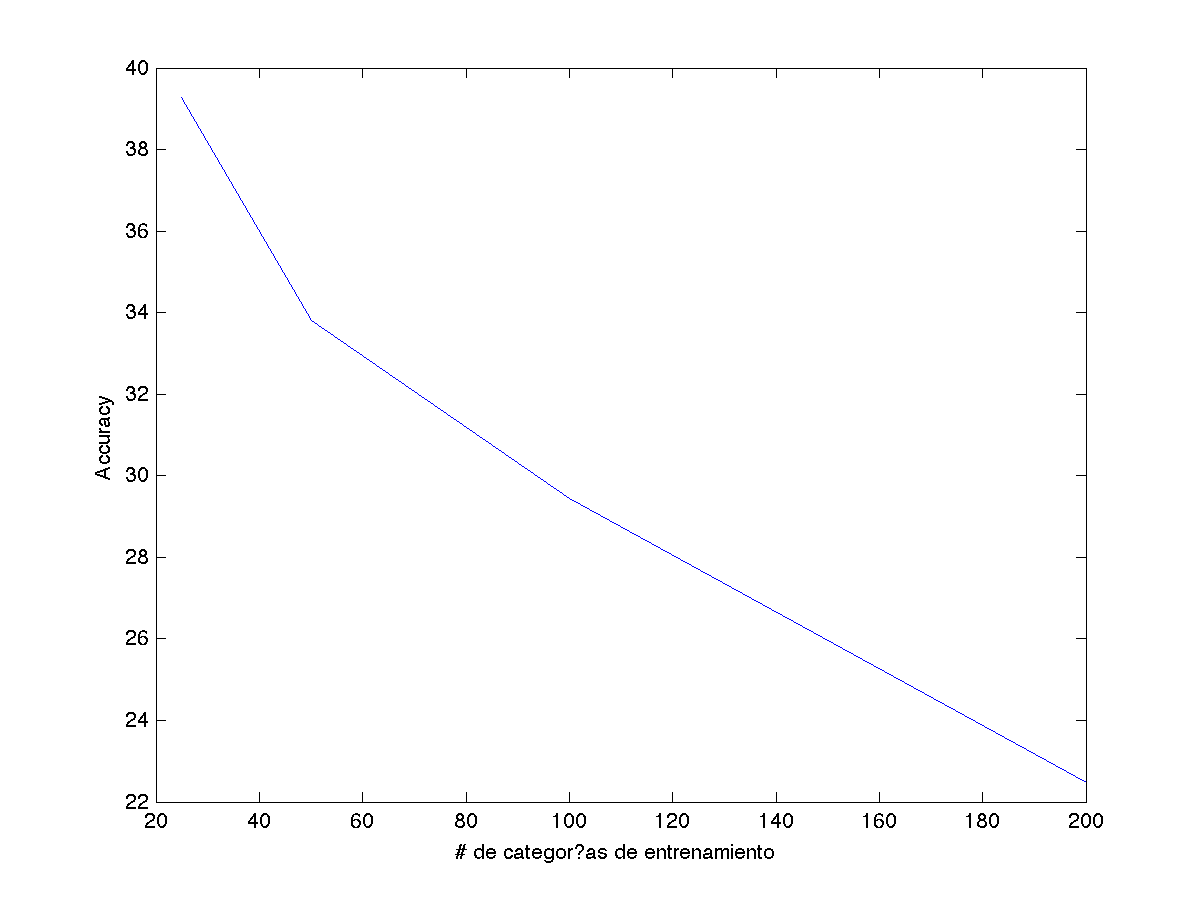
\includegraphics[scale = 0.4]{fig4catPHOW}
\end{center}
   \caption{Gráfica de precisión contra los números de categorías presentes en el modelo}
\end{figure}

También se presenta una tabla con los tiempos de duración comparativos de cada porción del algoritmo para cada uno de los modelos. Los resultados se pueden observar en la tabla 2.

%--------------Tabla Categorias
\begin{table*}
\caption{Tiempos comparativos para los modelos con variación de la variable \textit{conf.numClasses}}
\centering
\begin{tabular}{lcccl}
 & \multicolumn{4}{c}{\textit{Categorias}} \\
\multicolumn{1}{c}{\textit{Actividad}} & 25 & 50 & 100 & 200 \\ \hline
1. Setup data & 0.6536 s & 1.3144 s & 3.6759 s & 7.1407 s \\ \hline
2. Train vocabulary & 29.3394 s & 29.9198 s & 30.8575 s & 32.3204 s \\ \hline
3. Compute spatial histograms & 581.1571 s & 1208.9 s & 2435.3 s & 5102.0 s \\ \hline
4. Compute feature map & 0.8232 s & 1.6064 s & 3.2394 s & 7.1995 s \\ \hline
5. Train SVM & 37.1015 s & 109.8803 s & 376.7111 s & 1521.2 s \\ \hline
6. Test and Evaluate SVM & 0.3965 s & 1.0417 s & 2.0489 s &  \\ \hline
\end{tabular}
\end{table*}

\subsection{ \textit{C. Imágenes de entrenamiento}}

Similar a como se ha realizado en los métodos anteriores para determinar la influencia de los cambios de una variable sobre los modelos, en este se evalúan los modelos en los cuales solo cambia la variable \textit{conf.numTrain}. Lo anterior se logra al analizar los modelos con 200 categorías, y configuración espacial de [2,4]. A continuación se presenta una figura que resume los resultados obtenidos:

\begin{figure}
\begin{center}
   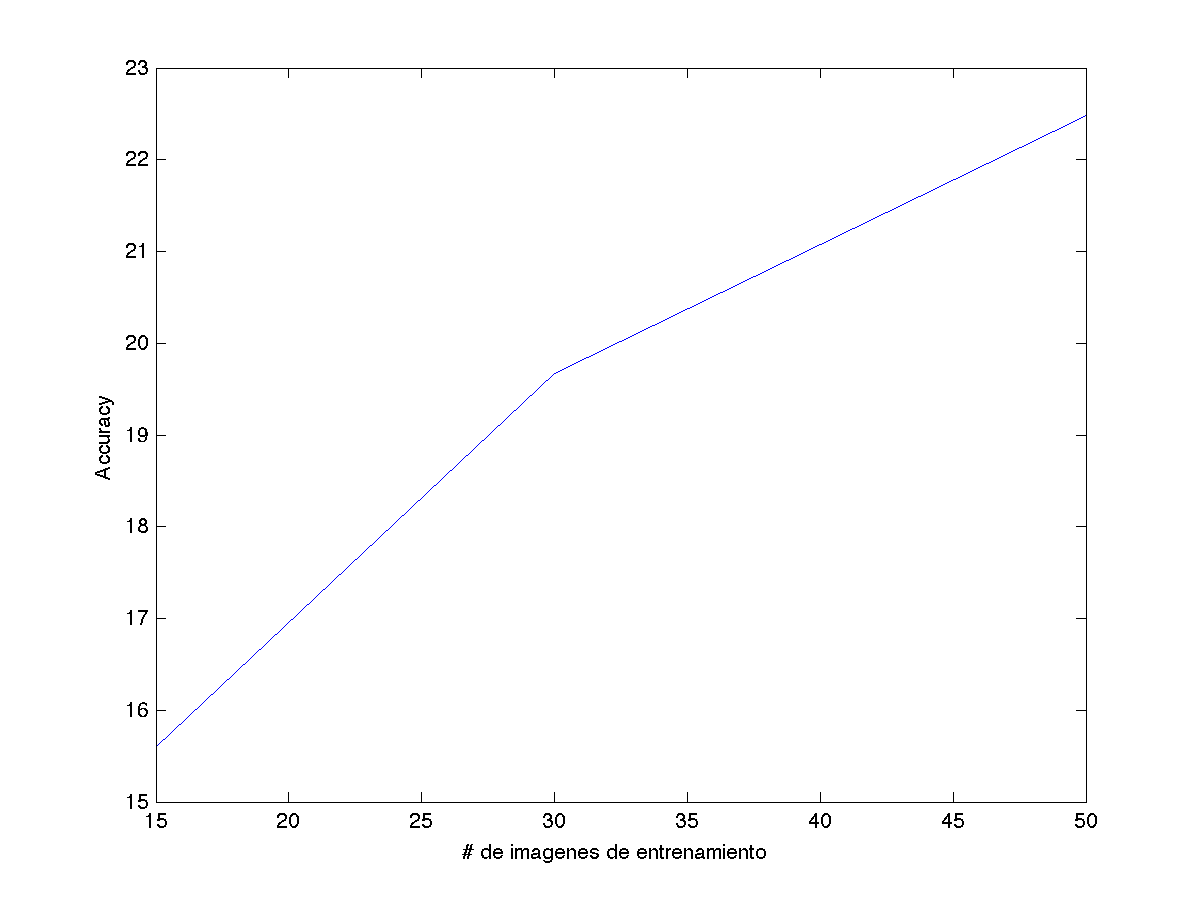
\includegraphics[scale = 0.4]{fig3trainPHOW}
\end{center}
   \caption{Gráfica de precisión contra la cantidad de imágenes empleadas en el entrenamiento del modelo}
\end{figure}

Igualmente, se presenta los tiempos de duración de cada una de las porciones del algoritmo para las configuraciones de los modelos entrenados variando únicamente el número de imágenes empleadas en el entrenamiento. Dichos resultados se presentan en la tabla 3.

%-------------Tabla Training
\begin{table*}
\caption{Tiempos comparativos para los modelos con variación de la variable \textit{conf.numTrain}}
\centering
\begin{tabular}{lcccc}
 & \multicolumn{4}{c}{\textit{Imágenes de Entrenamiento}} \\
\multicolumn{1}{c}{\textit{Actividad}} & 15 & 30 & 50 & 100 \\ \hline
1. Setup data & 6.0241 s & 3.6630 s & 7.1407 s & 7.6429 s \\ \hline
2. Train vocabulary & 34.6274 s & 33.5722 s & 32.3204 s & 29.6592 s \\ \hline
3. Compute spatial histograms & 5063.3 s & 5092.6 s & 5102.0 s & 5119.1 s \\ \hline
4. Compute feature map & 7.3384 s & 7.2959 s & 7.1995 s & 6.3762 s \\ \hline
5. Train SVM & 0.7842 s & 0.7683 s & 1521.2 s & 2808.8 s \\ \hline
6. Test and Evaluate SVM & 1.7300 s & 3.4048  s & 34.5252 s & 18.6851 \\ \hline
\end{tabular}
\end{table*}

\subsection{ \textit{D. Recursos Computacionales}}
Además de evaluar los tiempos de computación necesarios para cada método, los recursos computacionales se evaluaron empleando el administrador de procesos para obtener información acerca de porcentaje del CPU empleado para desarrollar las tareas de Matlab, la memoria RAM empleada para dicho proceso, y la energía requerida para realizar los procesos. Los resultados se observan en la figura 14.

\begin{figure}
\begin{center}
   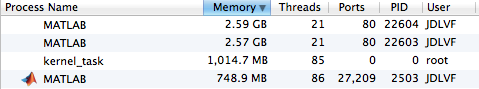
\includegraphics[scale = 0.437]{memory}
   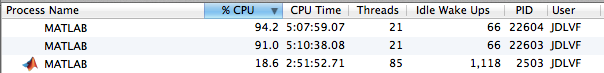
\includegraphics[scale = 0.35]{CPU}
   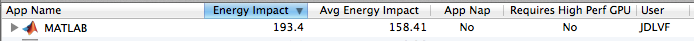
\includegraphics[scale = 0.305]{EnergyImp}
\end{center}
   \caption{Información del administrador de procesos demostrando el empleo de los recursos de RAM, CPU e impacto energético al emplear el software Matlab durante el procesamiento de los códigos}
\end{figure}

\section{\textbf{IV. Discusión}}
Los resultados obtenidos para la precisión de los modelos son regulares, ninguno supera el 40\%, lo cual indica que no está funcionando adecuadamente el descriptor seleccionado en la base de prueba. Esto se puede deber a que el descriptor fue desarrollado para Caltech-101, una base de datos sencilla, que posee objetos centrados, sin presencia de ruido en la imagen, y en posiciones estereotípicas. Inclusive, el mismo código en la base de datos de Caltech-101 posee resultados satisfactorios del 68.37\% de precisión (figura 15). 

\begin{figure}
\begin{center}
   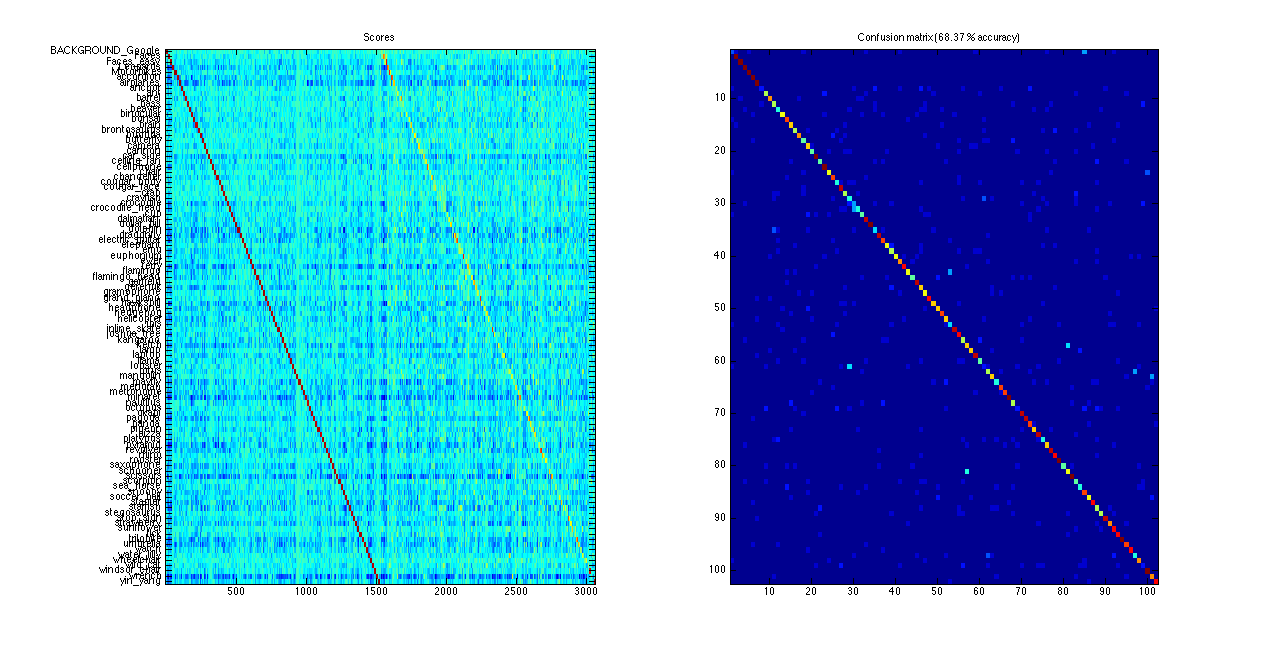
\includegraphics[scale = 0.2]{ConfusionMatrixCaltech}

\end{center}
   \caption{Matriz de confusiones para la base de datos Caltech-101 empleando PHOW}
\end{figure}

Ahora bien, la base de datos que se está empleado posee varios objetos en una imagen, con ruido en el fondo, y en diversas poses, acercamientos, y no necesariamente centrado, lo cual aumenta la dificultad del problema. En la figura 15 se observa una diagonal muy definida, es decir, existe poca confusión en las categorías. Comparativamente, en todas las matrices de confusión de los modelos entrenados se observa que la diagonal es tenue, en especial en los casos en los que se evalúan todas las categorías (200), y al realizar un acercamiento, evaluando únicamente 25 categorías, se observa que existe confusión para categorías como chihuahua, english springer, entle bucher, indian cobra, weimaraner, entre otros. A continuación se realizará la discusión de las variables individuales que fueron modificadas.

\subsection{ \textit{A. Número de divisiones espaciales}}
La variación de la precisión conforme al número de divisiones espaciales varía de forma parabólica, con la concavidad hacia abajo. Como tal presenta un punto máximo alrededor de la configuración [2,4], hacia ambos lados de la curva, decrece, sin embargo, a medida que se aumenta el número de divisiones espaciales la precisión decrece con mayor velocidad. Esto se puede ocasionar debido a que se fracciona demasiado la imagen, perdiendo la información importante de los píxeles circundantes al pixel central. 
Con relación al tiempo, el proceso que mayor variación de tiempo tuvo al cambiar esta variable fue el entrenamiento del clasificador Support Vector Machine, a medida que se incrementa el número de particiones en la imagen, se debe procesar aun más información. Lo anterior podría explicar que el tiempo para la configuración espacial [8,16] corresponda a más del triple de aquellos modelos con configuración [1,2] y [2,4]. La evaluación del Support vector machine, también aumenta, sin embargo, en ninguno de los casos supera un segundo, por lo cual se toma como no significativo. 

\subsection{ \textit{B. Número de categorías}}
La disminución del número de categorías refleja un aumento significativo en la precisión obtenida. Se podría modelar mediante una función exponencial. Este comportamiento se debe a que a medida que se disminuye el número de categorías, el clasificador tiene menos probabilidades de fallar al asignar una categoría. El cambio del número de categorías es el más significativo, tal vez se deba a su más amplio rango de variación. Para 200 categorías, la precisión es de 22.48\%, mientras que para 25 categorías, la precisión es de 39.28\%. Aunque ninguna es muy alta, la precisión con 25 categorías casi duplica la precisión de 200 categorías. Sin embargo, corresponde aproximadamente al 12\% de la muestra de 200 categorías. 

Debido a que cambia la cantidad de datos que se evalúan al cambiar el número de categorías, en especial en la configuración que se está evaluando el modelo, a medida que se aumenta una categoría aumenta en 50 imágenes la base de entrenamiento. Es por ello que en cuanto a tiempo se observa que Setup Data entre los métodos varía cerca a un segundo. Nuevamente, el entrenamiento del SVM es el que demuestra la mayor variación, el tiempo de entrenamiento para el modelo con 200 categorías corresponde a más de cuatro veces el tiempo de entrenamiento del modelo con 100 categorías.
 
También se observa un gran incremento en el tiempo de cálculo de los histogramas de espacio; aquel con 200 categorías duplica el tiempo del modelo con 100 categorías. En esta variable se observa mayor variación en los tiempos que en la variable de distribución espacial. Probablemente se relacione con lo que se mencionó anteriormente, a medida que se aumenta en una categoría, se aumenta por 50 imágenes la base de entrenamiento, incrementando los datos que se deben procesar, y por ende el tiempo de procesamiento. 

\subsection{ \textit{C. Tamaño de la base de datos de entrenamiento}}

El aumento del tamaño de la base de datos de entrenamiento conlleva a un aumento en la precisión del modelo. La curva parecería describir una función logarítmica. El aumento es significativo, con 15 imágenes se tiene una precisión del 15.60\%, y al aumentar la base a 50 imágenes, se obtiene una precisión del 22.48\%, aumentando en 7\% al aumentar por 35 imágenes la base de datos.Esto se debe a que a medida que el modelo tenga más imágenes de donde aprender, la clasificación de una nueva imagen será mucho más precisa 

En cuanto al tiempo de procesamiento de los datos, los cambios más significativos se observan en el entrenamiento del SVM, como en las categorías anteriores, donde se duplica el tiempo de entrenamiento cuando se utilizan 100 imágenes de entrenamiento por categoría comparado con el modelo que emplea 50 imágenes de entrenamiento por categoría. Existen unos tiempos que no parecerían concordar con los demás, en especial los del modelo de 30 imágenes por categoría, es posible que se deba a que la capacidad de procesamiento del computador estuvo limitada debido al uso concomitante de otros programas. 

\section{\textbf{IV. Conclusiones}}

Los modelos desarrollados que implementan PHOW para la clasificación de imágenes de la base de datos Imagenet Tiny no resultan tan satisfactorios como cuando se emplea PHOW sobre la base de datos Caltech-101. Esto se debe a la complejidad de la base de datos Imagenet respecto a la base de datos Caltech-101. Como tal, las imágenes de Imagenet presentan mayores variaciones en cuanto a los ángulos en los cuales la imagen es capturada, la posición del objeto en la imagen, hay ruido en el fondo, además de que incluye muchos animales, que son articulados y no rígidos también dificulta la tarea, debido a que PHOW requiere rigidez en las imágenes. 
Sin embargo, al modificar las variables del número de categorías, el número de imágenes de entrenamiento, y la distribución espacial se logra modificar la precisión alcanzada del modelo que implementa PHOW. Al modificar únicamente las categorías, aumentándolas, la precisión del modelo disminuye debido a que se aumenta la complejidad de distinción entre categorías. Al aumentar el número de imágenes en la base de entrenamiento, aumenta la precisión del modelo debido a que se entrena con más información, alcanzando una mayor especificidad en cada categoría. 
Al aumentar o disminuir la distribución espacial de [2,4], el desempeño del modelo disminuye, debido a su comportamiento similar a una parábola. Si se aumenta la distribución no se tendrá la información suficiente de los píxeles circundantes al pixel central. Y, en el caso contrario, si se disminuye en número, habrá un exceso de información circundante, la cual actuará como ruido al momento de clasificar la imagen. 
\subsection{ \textit{A. Limitaciones y Mejoras}}

El tamaño de la base de datos es una limitación, para 200 categorías, 100 imágenes es muy poco para entrenar, en particular si son tan diversas entre sí dentro de la misma categoría. Adicionalmente, el método que se está empleando supone rigidez en los objetos, lo cual no se logra cuando se clasifican animales debido a que estos son articulados y pueden aparecer en cualquier posición dentro de la imagen, lo cual aumenta la dificultad del problema. Tal vez para este problema sería más eficiente emplear Poselets o un modelo basado en partes, que son más complejos, pero corresponderían mejor a las imágenes que se están utilizando. También se podría intentar con diferentes tipos de clasificadores, como árboles de decisiones, que permiten clasificar distintas categorías en un mismo tiempo.

 

\section{\textbf{Referencias}}
\begin{enumerate}[label={[\arabic*]}]
\item R. Szeliski, “Chapter 14.4 Bag of Words,” in Computer Vision: Algorithm and Applications, Springer, 2010, pp.235-253.\\
\item L. Fei-Fei, R. Fergus, P. Perona, Learning generative visual models from few training examples: an incremental Bayesian approach tested on 101 object categories. IEEE. CVPR 2004, Workshop on Generative-Model Based Vision, 2004.
\item A. Vedaldi, B Fulkerson, An Open and Portable Library of Computer Vision Algorithms. 2008. retrieved from: \url{http://www.vlfeat.org/}
\item D. Forsyth, J. Ponce, Computer Vision: A Modern Approach, Upper Saddle River: Pearson, 2003, pp. 68-83.\\




\end{enumerate}



\end{document}
